% \documentclass{beamer}
\documentclass[aspectratio=169]{beamer}
\usepackage{hyperref}
%% \usepackage[CJKmath=true, AutoFakeBold = true]{xeCJK}
\usepackage[T1]{fontenc}
%% \setCJKmainfont{AR PL KaitiM GB} % Set Chinese font to KaiTi (calligraphy style)

% Other packages
\usepackage{latexsym,xcolor,multicol,booktabs,calligra}
% \usepackage{amssymb,amsfonts,amsmath,amsthm,mathrsfs,mathptmx} % Common math packages
\usepackage{amsmath,amssymb,amsfonts,mathrsfs} % Best mathematical packages
\usepackage{newtxtext,newtxmath} % Times-like font package for text and mathematics

\usepackage{graphicx,pstricks,listings,stackengine}
\usefonttheme[onlymath]{serif} % Use serif font for equations (better appearance)

% Other packages (new)
\usepackage[linesnumbered,ruled,vlined]{algorithm2e}
\SetKwComment{Comment}{$\triangleright$ }{} % The argument will be surrounded by /* ... */
\SetAlCapFnt{\footnotesize} % Make caption text smaller
\SetAlCapNameFnt{\footnotesize} % Make "Algorithm" label smaller
\usepackage{graphicx} % Enables inclusion and scaling of images (\includegraphics)
\usepackage{animate} % Provides support for frame-by-frame animations (\animategraphics)
\usepackage{subcaption} % Provides support for subfigures (subfigure environment with captions)
\usepackage{fontawesome5} % Provides scalable vector icons (Font Awesome 5 icons)
\usepackage{caption}
\captionsetup{
    font=footnotesize, % Reduce caption text size
    skip=5pt, % Space between figure and caption
    belowskip=0pt % Space below the caption (reduces gap after caption)
}
\usepackage{forest}
\usepackage[table]{xcolor}

% Water mark
\usepackage{tikz}
\usepackage{eso-pic}
\AddToShipoutPictureFG{
\begin{tikzpicture}[remember picture,overlay]
\node[
    rotate=45,
    scale=8,
    text opacity=0.08
] at (current page.center) {PUCP};
\end{tikzpicture}
}

% Adjusts horizontal margins of the slide content
% \setbeamersize{
%     text margin left=20pt, % Left margin of the slide content
%     text margin right=20pt % Right margin of the slide content
% }

\newcommand{\source}[1]{\par\tiny Source: #1} % Defines a reusable command to display the image/table source in small font below the caption

\renewcommand{\today}{\number\year-\number\month-\number\day}
\renewcommand{\alert}[1]{\textbf{\color{swufe}#1}}
\newcommand{\alertplain}[1]{{\color{swufe}#1}}

% Title page setup
\author[Edwin A. M. et al.]{\underline{Edwin Alvarez-Mamani} \inst{1,2}, Deybis Paucar Pinto \inst{1, 2}, Florian Buettner \inst{3}, Alfredo J. Ibañez \inst{1}, Madina Mansurova \inst{1}}
% \author[Topics]{Topics}

% Goethe-University Frankfurt and the German Cancer Consortium (DKTK)/German Cancer Research Center (DKFZ).

\title[Aligning Metabolomic Networks via Graph Learning...]{Aligning Metabolomic Networks via Graph Learning for Common Subnetwork Discovery}
% Custom title template with a styled box
\setbeamertemplate{title}{
    \makebox[\textwidth]{ % force horizontal centering
        \begin{beamercolorbox}[
            wd=1.0\textwidth,
            sep=1pt,
            center,
            rounded=true,
            shadow=false
        ]{title}
            \usebeamerfont{title}
            \inserttitle
        \end{beamercolorbox}
    }
}

% \subtitle{Jiangnan University Academic Report Beamer Template}
\institute[ICOBA-PUCP, UNSAAC ]{\footnotesize{\inst{1} \texttt{Institute for Omics Sciences and Applied Biotechnology, Pontificia Universidad Católica del Perú}} \\ \footnotesize{\inst{2} \texttt{Department of Informatics, Universidad Nacional de San Antonio Abad del Cusco}} \\ \footnotesize{\inst{3} \texttt{German Cancer Research Center, Goethe University Frankfurt and German Cancer Consortium}}}
% \institute[JNU]{\normalsize{\inst{1} School of Business \quad Jiangnan University \quad \textit{****@qq.com}}}

% \institute[ICOBA-PUCP, UNSAAC]{
%     
\includegraphics[width=0.15\linewidth]{../images/pucp.png}
% }

% \date{\today}
\date{\scriptsize June, 2026}

\usepackage{JNU}

% Defs
\def\cmd#1{\texttt{\color[RGB]{0, 0, 139}\footnotesize $\backslash$#1}}
\def\env#1{\texttt{\color[RGB]{0, 0, 139}\footnotesize #1}}

\lstset{
    language=[LaTeX]TeX,
    basicstyle=\ttfamily\footnotesize,
    keywordstyle=\bfseries\color[RGB]{0, 0, 139},
    stringstyle=\color[RGB]{50, 50, 50},
    numbers=left,
    numberstyle=\small\color{gray},
    rulesepcolor=\color{red!20!green!20!blue!20},
    frame=shadowbox,
}

\begin{document}

\begin{frame}
    \titlepage
    \begin{figure}[htpb]
        \begin{center}
            %% 
\includegraphics[width=0.55\linewidth]{../images/jiangnan_logo.png}
        \end{center}
    \end{figure}
\end{frame}

% \begin{frame}
%     \tableofcontents[sectionstyle=show,subsectionstyle=show/shaded/hide,subsubsectionstyle=show/shaded/hide]
%     % \tableofcontents[sectionstyle=show,subsectionstyle=hide,subsubsectionstyle=hide]
% \end{frame}

% Timing: Your total presentation length is 15 minutes, broken down as:  
% - 10-12 minutes of talking/presenting 
% - 2-4 minutes of Q&A with the audience 
% - 1 minute to transition to the next speaker 

% Quitar Outline

\section{Introduction}
    % Motivation and research gap
    % Problem formulation
    % Research question

    % \begin{frame}{Motivation} % NO
    %     Mass spectrometry is an analytical technique that is used to identify and quantify chemical compounds in a sample.

    %     \begin{figure}[htp!]
    %         \centering
    %         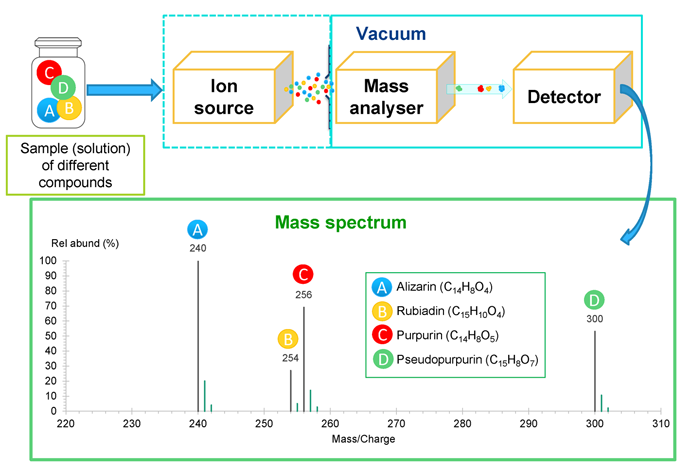
\includegraphics[
    %             width=0.45\linewidth,
    %             trim=0pt 0pt 0pt 0pt, % trim: left bottom right top
    %             clip
    %         ]{../images/ms_spectrum.png}
    %         \caption{Overall scheme of a mass spectrometer and formation of a mass spectrum.}
    %         \source{\url{https://sisu.ut.ee/heritage-analysis/52-mass-spectrometry}} 
    %         % \cite{putri2014mass}
    %         % \label{fig:my_image}
    %     \end{figure}

    %     \begin{note}
    %         {Introduce your self}
    %     \end{note}
    % \end{frame}

    % Motivation_ unta

    \begin{frame}{Acknowledgments}
        % 
        % The authors acknowledge the financial support provided by the Consejo Nacional de Ciencia, Tecnología e InnovaciónTecnológica (CONCYTEC–Prociencia) through funding project PE501086715-2024-PROCIENCIA. \newline

        Financial support was provided by CONCYTEC-Prociencia through project PE501086715-2024-PROCIENCIA. Also, I gratefully acknowledge the Pontificia Universidad Católica del Perú (PUCP) for the financial support provided for conference registration.

        \begin{figure}
            \centering
            \begin{subfigure}{0.4\textwidth}
                \centering
                
\includegraphics[
                    width=\linewidth,
                    trim=0pt 50pt 0pt 50pt, % trim: left bottom right top
                    clip
                ]{../images/PUCP_logo.png}
                % \caption{My image.}
                % \source{Author, 2024.}
            \end{subfigure}
            % \hfill
            \hspace{1cm}
            \begin{subfigure}{0.4\textwidth}
                \centering
                
\includegraphics[
                    width=\linewidth,
                    trim=0pt 130pt 0pt 150pt, % trim: left bottom right top
                    clip
                ]{../images/PROCIENCIA-LOGO.png}
                % \caption{My image.}
                % \source{Author, 2024.}
            \end{subfigure}
            % \caption{My image.}
            % \source{Author, 2024.}
            % \label{fig:my_image}
        \end{figure}

        \begin{note}
            {Introduce your self}
        \end{note}
    \end{frame}

    \begin{frame}{Problem formulation}
        % Targeted and untargeted analyses
        The mass spectrometry analysis includes two approach: \alert{targeted} analysis and \alert{untargeted} analysis.

        % \begin{itemize}
        %     \item \alert{Targeted approach:} the molecule of interest or m/z values (for MS and MS/MS) are predefined for quantitation of analytes present in a complex samples matrix. %, with high sensitivity, accuracy, and specificity
        %     \item \alert{Untargeted approach:} is the analysis to identify the unknowns in a sample, using parent ion and product or fragment ion analysis (MS/MS).
        % \end{itemize}

        \begin{columns}[b] % Option "c" centers vertically, while "t" aligns to the top.
            \begin{column}{0.59\textwidth}
                \begin{figure}[htp!]
                    \centering
                    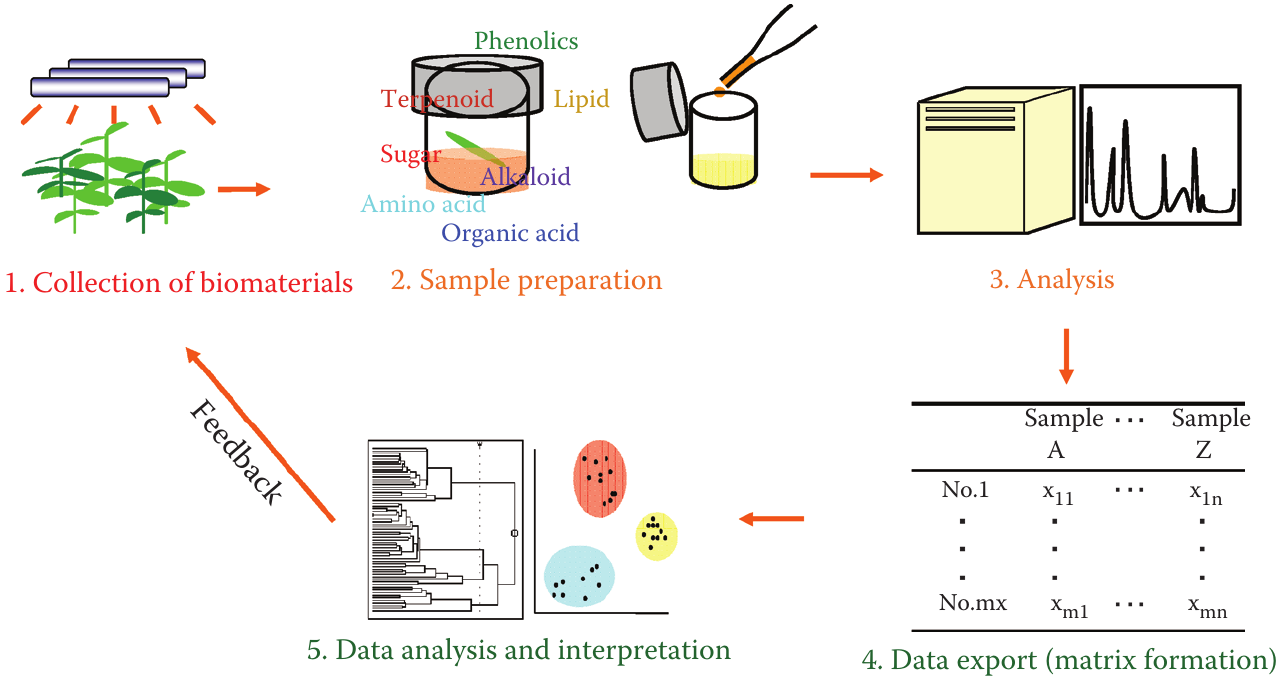
\includegraphics[
                        width=1.0\linewidth,
                        trim=0pt 0pt 0pt 0pt, % trim: left bottom right top
                        clip
                    ]{../images/metabolomics_workflow.png}
                    \caption{Metabolomics workflow \footnotemark[1].}
    
                    % Putri, S. P., \& Fukusaki, E. (Eds.). (2014). Mass spectrometry -based metabolomics: a practical guide. CRC Press.
                    % \source{\cite{putri2014mass}} 
                    % \label{fig:my_image}
                \end{figure}
            \end{column}
            \begin{column}{0.41\textwidth}
                \begin{figure}[htp!]
                    \centering
                    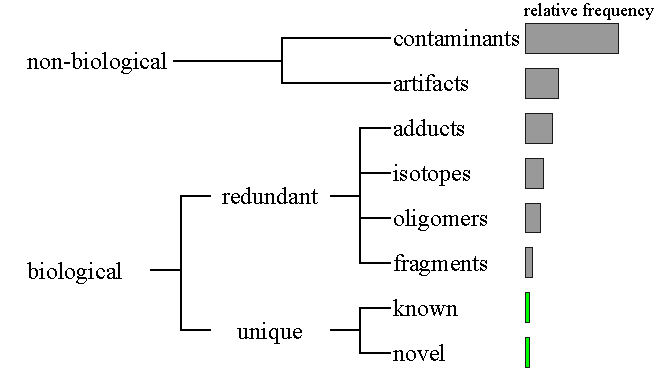
\includegraphics[
                        width=1.0\linewidth,
                        trim=0pt 0pt 0pt 0pt, % trim: left bottom right top
                        clip
                    ]{../images/untargeted_data.pdf}
                    \caption{Untargeted composition \footnotemark[2].}
                    
                    % Sindelar, M., \& Patti, G. J. (2020). Chemical discovery in the era of metabolomics. Journal of the American Chemical Society, 142(20), 9097-9105.
                    % \caption{Untargeted composition.}
                    % \source{Adapted from \cite{sindelar2020chemical}}
                    % \label{fig:my_image}
                \end{figure}
            \end{column}
        \end{columns}

        \footnotetext[1]{\tiny{Putri, S. P., \& Fukusaki, E. (Eds.). (2014). Mass spectrometry -based metabolomics: a practical guide.}}

        \footnotetext[2]{\tiny{Sindelar, M., \& Patti, G. J. (2020). Chemical discovery in the era of metabolomics.}}

        \begin{note}
            {Introduce your self}
        \end{note}
    \end{frame}

    % \begin{frame}{Untargeted mass spectrometry workflow}
    %     A data matrix (sample vs. metabolites) acquired from a mass spectrometry-based metabolomics study includes not only biological information but also technical noise. % There are several techniques for univariate or multivariate statistical analysis. Some statistical methods used are: Principal component analysis (PCA), Hierarchical cluster analysis (HCA), Correlation analysis (CA), Projection to latent structure regression (PLS-R), Projection to latent structure discriminant analysis (PLS-DA), and t-Test. It is very important to use and interpret the statistical result accurate \cite{putri2014mass}.

    %     \begin{note}
    %         {Introduce your self}
    %     \end{note}
    % \end{frame}

    \begin{frame}{Our objectives}
        % Aligning metabolomic networks for \alert{filter} mass spectrometry data via graph neural network models.
        Aligning metabolomic networks to filter relevant features from Mass Spectrometry (MS) data via Graph Neural Networks (GNNs). \newline

        % Filtering and detecting of significant changes between metabolomic networks using graph representation learning models and an anomaly detection algorithm to obtain reliable results in less time.

        % \begin{itemize}
        %     % \item Improve the detection of significant changes between metabolomic networks using Graph Neural Network (GNN) models and to obtain reliable results in less time.
        %     % \item Develop a pipeline for data processing and analysis.
        %     % \item Develop a pipeline for data processing and analysis.

        %     %% \item Develop a workflow for the analysis of metabolomic networks.
        %     %% \item Model metabolomic networks from mass spectrometry data.
        %     %% \item Implement GNN models to learn metabolite representations. % for network alignment tasks
        %     %% \item Evaluate the effectiveness of the proposed GNN-based alignment approach.
        %     % \item Comparison of the quality of node embeddings. % (generated by GNN models) for the analysis of metabolomic networks. % check
        %     % \item Evaluation of execution times in the generation and manipulation of embeddings.
        %     % \item Implement a web application for the analysis of metabolomic networks.
        %     % \item Develop a web application.

        %     \item Design a workflow for metabolomic network analysis.
        %     \item Construct metabolomic networks from Mz data.
        %     \item Develop Graph Neural Network models to learn metabolite representations.
        %     \item Assess the effectiveness of the proposed GNN-based approach for metabolomic network alignment.
        % \end{itemize}

        \begin{itemize}
            \item Construct metabolomic networks from MS data and identify shared features through network alignment.
            
            \item Apply GNN models to learn metabolite representations that capture the structural properties of metabolomic networks.
            
            \item Explore the potential of GNN-based alignment to integrate metabolomic datasets acquired on different days while mitigating batch effects.
        \end{itemize}

        \begin{note}
            {Introduce your self}
        \end{note}
    \end{frame}

\section{Background}
    % Metabolomics: GC-MS and LC-MS data
    % Graph representation: G=(V,E,X)G = (V, E, X)
    % G=(V,E,X)
    % Message passing in GNNs
    % GCN and GAT: key equations

    % \begin{frame}{Mass spectrometry (MS)}
    %     Mass spectrometry (MS) is a microanalytical technique used to detect and determine the amount of an analyte, it is also used to determine the elemental composition and some aspects of the molecular structure of an analyte. % \cite{watson2007introduction}

    %     \begin{figure}[htp!]
    %         \centering
    %         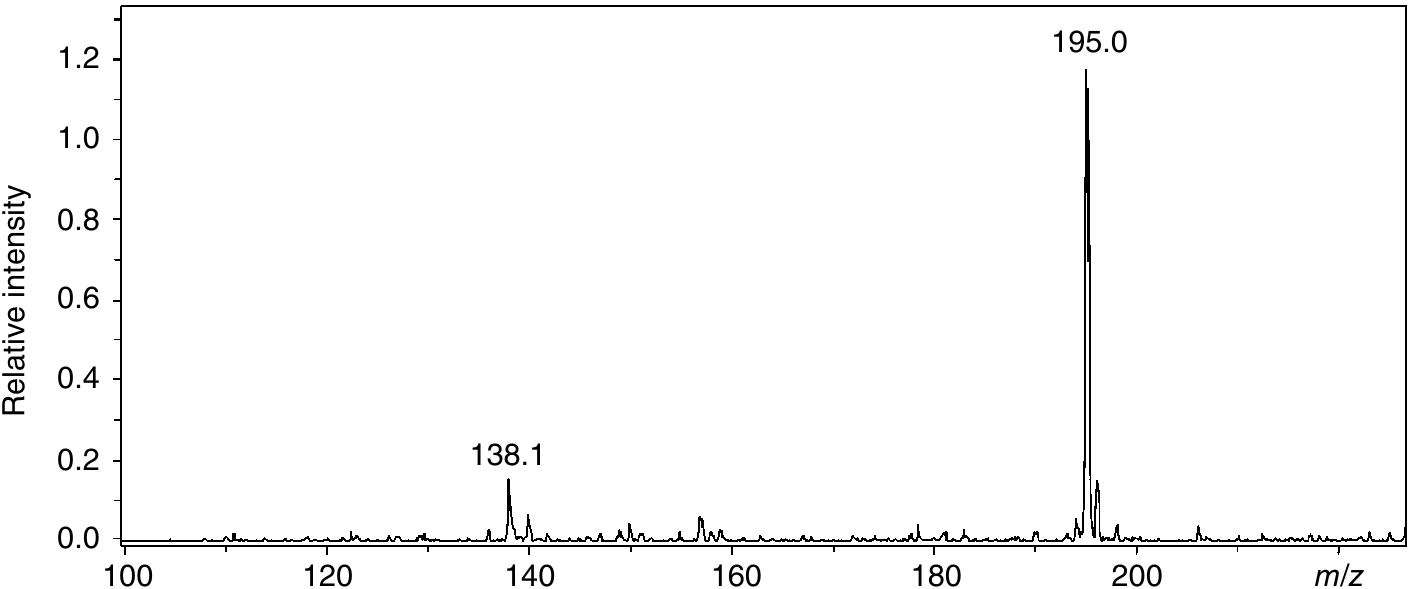
\includegraphics[
    %             width=0.8\linewidth,
    %             trim=0pt 0pt 0pt 0pt, % trim: left bottom right top
    %             clip
    %         ]{../images/mass_spectrum.png}
    %         \caption{Mass spectrum of caffeine obtained by electrospray ionization mass spectrometry (ESI‐MS) technique.}
    %         \source{\cite{smoluch2019mass}.}
    %         % \label{fig:my_image}
    %     \end{figure}

    %     \begin{note}
    %         {Introduce your self}
    %     \end{note}
    % \end{frame}

    % \begin{frame}{MS dataset format}
    %     \begin{figure}[htp!]
    %         \centering
    %         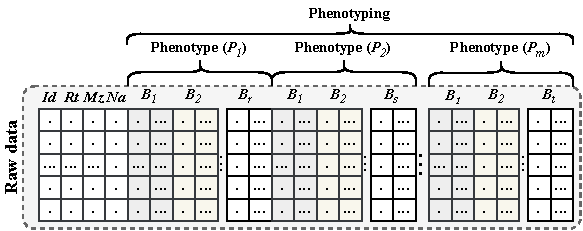
\includegraphics[
    %             width=0.8\linewidth,
    %             trim=0pt 0pt 0pt 0pt, % trim: left bottom right top
    %             clip
    %         ]{../images/raw_data.pdf}
    %         \caption{Aligned mass spectrometry data format.}
    %         % \source{Author, 2024.}
    %         % \label{fig:my_image}
    %     \end{figure}

    %     \begin{note}
    %         {Introduce your self}
    %     \end{note}
    % \end{frame}

    % \begin{frame}{Graph}
    %     A graph (network) is defined as $G = (V, E)$, where $V = \{v_1, v_2, ..., v_{n}\}$ is the nodes (or \textit{vertices}, or \textit{points}) set and $E = \{e_1, e_2, ..., e_{m}\}, e_i \in V \times V$ a set of edges (or \textit{lines}, or \textit{arcs}) formed by unordered pairs of nodes. \\

    %     % \vspace{2mm}
    %     % \scriptsize Number of nodes is denoted $|V|$. \\
    %     % Number of edges is denoted $|E|$.

    %     \begin{figure}
    %         \centering
    %         \begin{subfigure}{0.2\textwidth}
    %             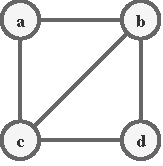
\includegraphics[width=\textwidth]{../images/graph_example.pdf}
    %             \caption{Input graph.}
    %             \label{fig:graph_example_}
    %         \end{subfigure}
    %         \hfill
    %         \begin{subfigure}{0.22\textwidth}
    %             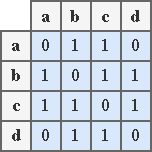
\includegraphics[width=\textwidth]{../images/graph_adjacency_matrix.pdf}
    %             \caption{Adjacency matrix.}
    %             \label{fig:graph_adjacency_matrix_}
    %         \end{subfigure}
    %         \hfill
    %         \begin{subfigure}{0.22\textwidth}
    %             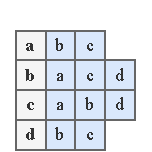
\includegraphics[width=\textwidth]{../images/graph_adjacency_list.pdf}
    %             \caption{Adjacency list.}
    %             \label{fig:graph_adjacency_list_}
    %         \end{subfigure}
    %         \hfill
    %         \begin{subfigure}{0.22\textwidth}
    %             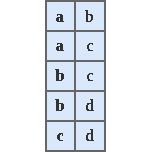
\includegraphics[width=\textwidth]{../images/graph_list_edge.pdf}
    %             \caption{Edge list.}
    %             \label{fig:graph_list_edge_}
    %         \end{subfigure}
    %         \caption{Graph representations.}
    %         \label{fig:graph_representation_}
    %     \end{figure}

    %     \begin{note}
    %         {Introduce your self}
    %     \end{note}
    % \end{frame}

    \begin{frame}{Graph Neural Network (GNN)}
        It is a function $f: (A, X) \rightarrow Z$ that maps each node $v \in V$ of a graph $G = (V, E)$ to a low-dimensional embedding $z_v \in \mathbb{R}^{d}$ ($d \ll |V|$). \\
        
        % Here $A \in \mathbb{R}^{|V| \times |V|}$ is the adjacency matrix, $X \in \mathbb{R}^{|V| \times C}$ is the node feature matrix, $C$ denotes the feature dimensionality, and $Z = H^{(L)} \in \mathbb{R}^{|V| \times d}$ is the final embedding matrix obtained after $L$ layers, with $H^{(0)} = X$.
        
        \begin{figure}[htp!]
            \centering
            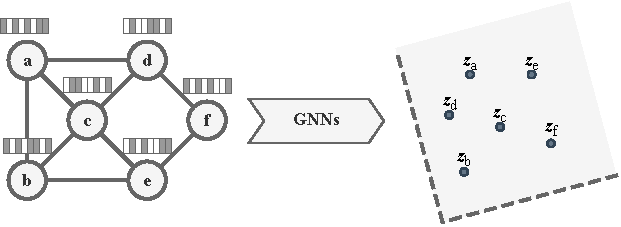
\includegraphics[
                width=0.8\linewidth,
                trim=0pt 0pt 0pt 0pt, % trim: left bottom right top
                clip
            ]{../images/graph_neural_networks.pdf}
            \caption{GNNs scheme.}
            % \source{}
            % \label{fig:my_image}
        \end{figure}

        \begin{note}
            {Introduce your self}
        \end{note}
    \end{frame}

    \begin{frame}{Graph aligment problem}
        % Let two graphs $G_1 = (V_1, E_1)$, $G_2 = (V_2, E_2)$. %, where $V_1$ and $V_2$ denote the sets of nodes, and $E_1$ and $E_2$ denote the sets of edges.

        % The graph alignment problem consists of finding a mapping $\pi: V_1 \to V_2$, such that each node $v \in V_1$ is assigned to a corresponding node $\pi(v) \in V_2$. %, maximizing a similarity criterion that captures structural and/or semantic correspondence between the two graphs.

        % Let $G_1 = (V_1, E_1)$ and $G_2 = (V_2, E_2)$ be two graphs. The node alignment problem aims to identify a correspondence between the node sets of two graphs through a mapping function:

        % Let $G_1 = (V_1, E_1)$ and $G_2 = (V_2, E_2)$ be two graphs. The goal is to identify a correspondence between the nodes in $V_1$ and those in $V_2$ through a mapping function:

        Let $G_1 = (V_1, E_1)$ and $G_2 = (V_2, E_2)$ be two graphs. The goal is to align their nodes through a mapping function $\mathbf{\pi : V_1 \rightarrow V_2}$, where each node $v \in V_1$ is mapped to its corresponding node $\pi(v) \in V_2$.

        \begin{figure}[htp!]
            \centering
            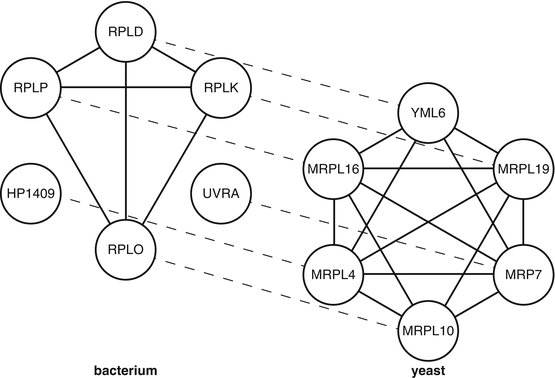
\includegraphics[
                width=0.5\linewidth,
                trim=0pt 0pt 0pt 0pt, % trim: left bottom right top
                clip
            ]{../images/graph_alignment_problem.png}
            \caption{Node alignment.}
            \source{\url{https://link.springer.com/rwe/10.1007/978-1-4419-9863-7_992}}
            % \label{fig:my_image}
        \end{figure}

        \begin{note}
            {Introduce your self}
        \end{note}
    \end{frame}

    \begin{frame}{Base GNN model}
        % \texttt{T-GAE}: Transferable Graph Autoencoder for Network Alignment \cite{he2024t}.
        \texttt{T-GAE}: Transferable Graph Autoencoder for Network Alignment\footnotemark[3]
        
        % \scriptsize (He, J., Kanatsoulis, C., \& Ribeiro, A., 2024)

        \begin{figure}[htp!]
            \centering
            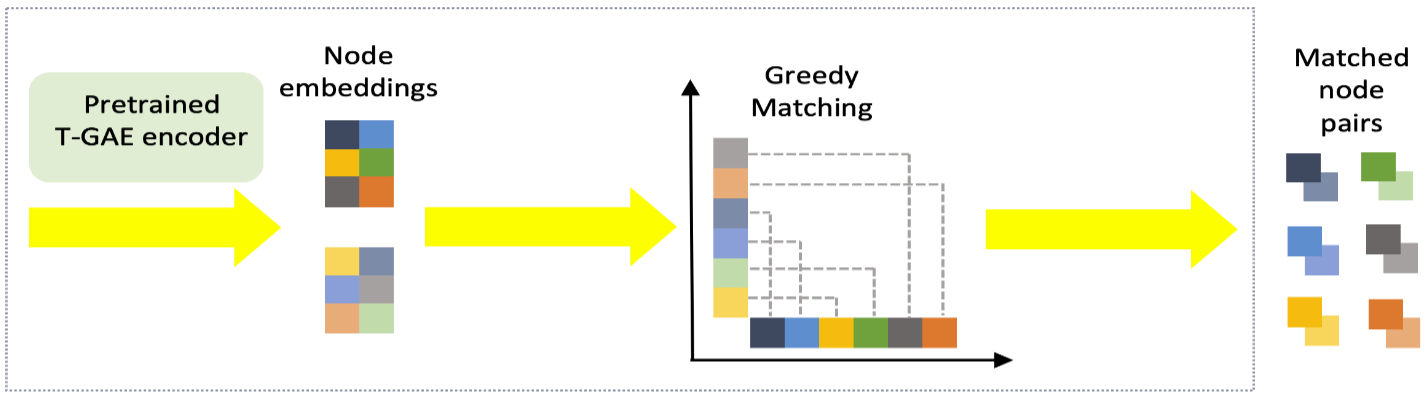
\includegraphics[
                width=0.9\linewidth,
                trim=0pt 0pt 0pt 0pt, % trim: left bottom right top
                clip
            ]{../images/T-GAE.png}
            \caption{\texttt{T-GAE} encoder.}
            % \source{Author, 2024.}
            % \label{fig:my_image}
        \end{figure}

        \footnotetext[3]{\tiny{He, J., Kanatsoulis, C., \& Ribeiro, A. (2024). T-gae: Transferable graph autoencoder for network alignment.}}

        \begin{note}
            {Introduce your self}
        \end{note}
    \end{frame}

\section{Method}
    % Metabolomic network construction
    % T-GAE architecture
    % Network alignment via KNN

    \begin{frame}{Mass spectrometry data}
        \begin{figure}[htp!]
            \centering
            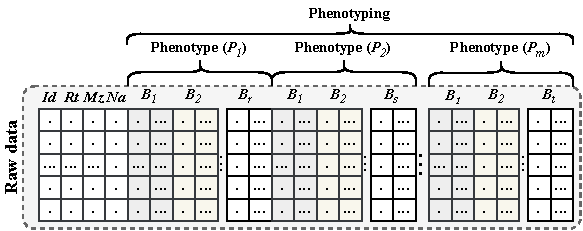
\includegraphics[
                width=0.8\linewidth,
                trim=0pt 0pt 0pt 0pt, % trim: left bottom right top
                clip
            ]{../images/raw_data.pdf}
            \caption{Dataset format.}
            % \source{Author, 2024.}
            % \label{fig:my_image}
        \end{figure}

        \begin{note}
            {Introduce your self}
        \end{note}
    \end{frame}

    \begin{frame}{Method}
        \begin{figure}[htp!]
            \centering
            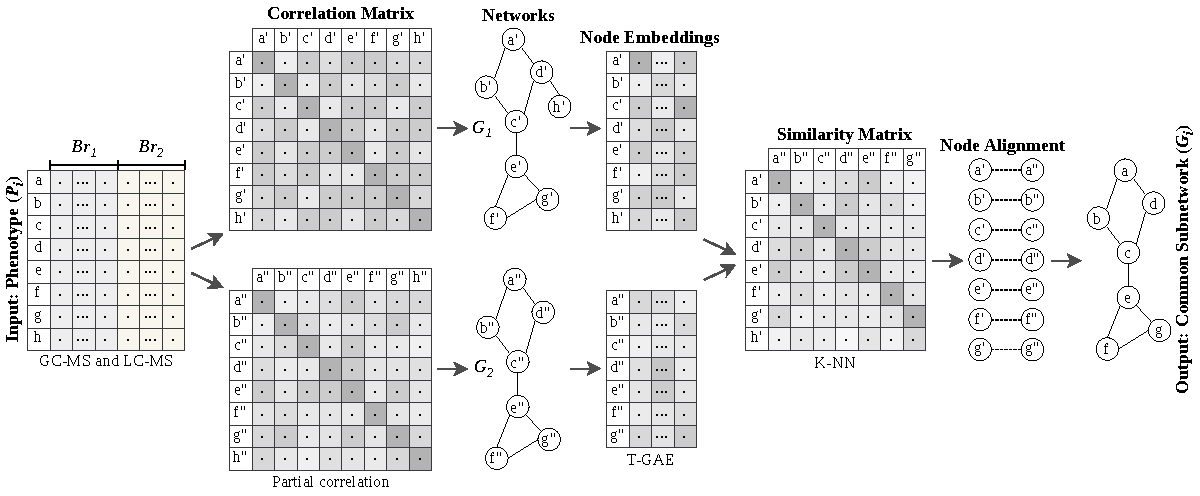
\includegraphics[
                width=1.0\linewidth,
                trim=0pt 0pt 0pt 0pt, % trim: left bottom right top
                clip
            ]{../images/Method_NA.pdf}
            \caption{Our workflow.}
            % \source{Author, 2024.}
            % \label{fig:my_image}
        \end{figure}

        \begin{note}
            {Introduce your self}
        \end{note}
    \end{frame}

    % \begin{frame}{Method overview}
    %     % \begin{enumerate}
    %     %     \item \textbf{Correlation estimation:} A correlation matrix is computed using partial correlation coefficients to capture direct relationships between metabolites while controlling for the influence of other variables.
    %     %     \item \textbf{Metabolic network construction:} A metabolic network is generated in which an edge is established between two nodes when the absolute correlation coefficient satisfies $|\text{coef}| \geq 0.5$. Node attributes incorporate transformed retention time ($Rt$), mass-to-charge ratio ($Mz$), and signal intensity measurements.
    %     %     \item \textbf{Graph representation learning:} Node embeddings are learned using the \texttt{T-GAE} architecture, which integrates \texttt{GIN} and \texttt{GINE} graph neural network layers to capture both topological and attribute information.
    %     %     \item \textbf{Network alignment:} A node similarity matrix is computed using the K-Nearest Neighbors (\texttt{KNN}) algorithm to identify correspondences between metabolites across different metabolic networks.
    %     % \end{enumerate}

    %     \begin{enumerate}
    %         \item \alert{Correlation estimation:} compute the partial correlation matrix $P = [\rho_{ij}]$ from mass espectrometry data.
    %         \item \alert{Network construction:} build a metabolic network using a correlation threshold ($|\rho_{ij}| \geq 0.5$), incorporate node features (like $Rt$, $Mz$, $Avg\; intensities$) and edge features (like $|\rho_{ij}|$, $\operatorname{sign}(\rho_{ij})$).
    %         \item \alert{Graph representation learning:} learn node embeddings with the \texttt{T-GAE} architecture based on \texttt{GIN} and \texttt{GINE} layers.
    %         \item \alert{Network alignment:} identify metabolite correspondences using a \texttt{KNN}-based similarity matrix.
    %     \end{enumerate}

    %     \begin{note}
    %         {Introduce your self}
    %     \end{note}
    % \end{frame}

\section{Experiments}
    % Dataset
    % Baseline methods
    % Evaluation metrics
    \begin{frame}{Experiments setup} % {Hardware/software}
        % The experiments were run on an AMD Ryzen Threadripper PRO 5955WX computer with 128 cores, 256 GB of RAM, 2x NVIDIA RTX A6000 with 48 GB of VRAM. The source code was implemented in \texttt{Python} with \texttt{Scikit-learn} and \texttt{PyTorch Geometric}.
        The experiments were run on computer with 128 cores, 256 GB of RAM, 2x NVIDIA RTX A6000 with 48 GB of VRAM. The source code was implemented in \texttt{Python} with \texttt{Scikit-learn} and \texttt{PyTorch Geometric}.

        \begin{table}[htp!]
            \footnotesize % \scriptsize
            \centering
            \caption{Experiments setup.}
            % \label{tab:table1}
            \begin{tabular}{@{}ll@{}}\toprule
                Features & Values \\\midrule
                % Node embedding & \texttt{T-GAE} \\
                GNNs architectures & \texttt{T-GAE} with \texttt{GIN}, \texttt{GINE} encoders \\
                Embedding dimensions & 16, 32, 64 \\ %, 256, 512 \\
                Optimizer & Adam with $lr=10^{-4}$, $weight\_decay=5 \times 10^{-4}$ \\
                Early stopping & $patience=10$ \\
                Epochs & 100 \\\midrule
                Node features & $Mz$, $Rt$, $\operatorname{log}(Avg\; intensities)$, $Std\; intensities$, $Cv\; intensities$ \\
                Edge features & $|\rho_{ij}|$, $\operatorname{sign}(\rho_{ij})$, $\rho_{ij}^{2}$ \\\midrule
                Dataset & Cocoa, Mentos, Leaf \\\bottomrule
            \end{tabular}
        \end{table}

        \begin{note}
            {Introduce your self}
        \end{note}
    \end{frame}

    \begin{frame}{Dataset}
        \begin{columns}[t] % Option "c" centers vertically, while "t" aligns to the top.
            \begin{column}{0.4\textwidth}
                These 3 datasets were used in the experiments. \\
        
                \begin{itemize}
                    \item Cocoa \footnotemark[4] (\small{from ICOBA-PUCP)}
                    \item Mentos \footnotemark[5] (\small{from ICOBA-PUCP)}
                    % \item Mutant \cite{buettner2017non}
                    % \item Leaf  \cite{gonzalez2023climate}
                    \item Leaf \footnotemark[6]
                    
                    % \item Synthetic
                \end{itemize}
            \end{column}
            
            \begin{column}{0.6\textwidth}
                \begin{figure}[htp!]
                    \centering
                    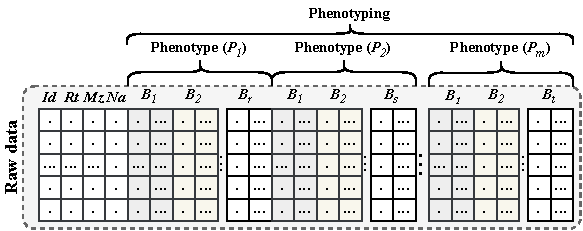
\includegraphics[
                        width=1.0\linewidth,
                        trim=0pt 0pt 0pt 0pt, % trim: left bottom right top
                        clip
                    ]{../images/raw_data.pdf}
                    \caption{Mass spectrometry data format.}
                    % \source{Author, 2024.}
                    % \label{fig:my_image}
                \end{figure}
            \end{column}
        \end{columns}

        \footnotetext[4]{\tiny{Cocoa dataset, available at: Poster number 1259 by Vanessa Jessenia Mayorga Martino.}}

        \footnotetext[5]{\tiny{Alvarez-Mamani, E., Buettner, F., Beltran-Castanon, C. A., \& Ibanez, A. J. (2024). Exploratory analysis of metabolic changes using mass spectrometry data and graph embeddings.}}
        % Alvarez-Mamani, E., Buettner, F., Beltran-Castanon, C. A., & Ibanez, A. J. (2024). Exploratory analysis of metabolic changes using mass spectrometry data and graph embeddings. Scientific reports, 14(1), 29570.

        \footnotetext[6]{\tiny{González-Teuber, M., Palma-Onetto, V., Aguirre, C., Ibáñez, A. J., \& Mithöfer, A. (2023). Climate change-related warming-induced shifts in leaf chemical traits favor nutrition of the specialist herbivore Battus polydamas archidamas.}}
        
        % González-Teuber, M., Palma-Onetto, V., Aguirre, C., Ibáñez, A. J., & Mithöfer, A. (2023). Climate change-related warming-induced shifts in leaf chemical traits favor nutrition of the specialist herbivore Battus polydamas archidamas. Frontiers in Ecology and Evolution, 11, 1152489.

        % \begin{table}[htp!]
        %     % \scriptsize
        %     \centering
        %     \caption{Datasets.}
        %     % \label{tab:table1}
        %     \begin{tabular}{@{}llrrrr@{}}
        %         \toprule
        %         Dataset & Type network & \#Nodes  & \#Edges & \#Features & \#Anchors/Pairs \\
        %         \midrule
        %         Douban Online & Social    & $3\,906$ & $1\,632$ & $538$ & $1\,118$  \\
        %         Douban Offline & Social    & $1\,118$   & $3\,022$  & $538$ & $1\,118$ \\\midrule
        %         ACM & Citation  & $9\,916$ & $44\,808$ & $17$ & $6\,325$  \\
        %         DBLP & Citation  & $9\,872$ & $39\,561$  & $17$ & $6\,325$  \\\bottomrule 
        %     \end{tabular}
        % \end{table}

        \begin{note}
            {Introduce your self}
        \end{note}
    \end{frame}

    % \begin{frame}{Experiments setup}

    %     \begin{table}[htp!]
    %         % \scriptsize
    %         \centering
    %         \caption{Experiments setup.}
    %         % \label{tab:table1}
    %         \begin{tabular}{@{}ll@{}}\toprule
    %             Features & Values \\\midrule
    %             Node embedding & 
    %             \texttt{T-GAE} \\
    %             Architectures & \texttt{GIN}, \texttt{GINE} \\
    %             Dimensions & 16, 32, 64 \\ %, 256, 512 \\
    %             Optimizer & Adam with $lr=10^{-4}$, $weight\_decay=5 \times 10^{-4}$ \\
    %             Early stopping & $patience=10$ \\
    %             Epochs & 100 \\\midrule
    %             Node features & $Mz$, $Rt$, $\operatorname{log}(Avg\; intensities)$, $Std\; intensities$, $Cv\; intensities$ \\
    %             Edge features & $|\rho_{ij}|$, $\operatorname{sign}(\rho_{ij})$, $\rho_{ij}^{2}$ \\\midrule
    %             Dataset & Cocoa, Mentos, Leaf, Synthetic \\\bottomrule
    %         \end{tabular}
    %     \end{table}

    %     \begin{note}
    %         {Introduce your self}
    %     \end{note}
    % \end{frame}

\section{Results}
    \begin{frame}{Metabolomic networks}
        \begin{table}[htp!]
            \footnotesize % \scriptsize
            \centering
            \caption{Cocoa dataset.} % December
            % \label{tab:table1}
            \begin{tabular}{@{}lcrrrcr@{}}\toprule
                Group & Subgroup & $|V|$  & $|E|$ & Density & Is connected? \\\midrule
                DryAmazonas    &	$1$ &	$559$	& $103\,333$ &	$0.662557$ &	True & \\
                DryAmazonas    &	$2$ &	$559$	& $104\,793$ &	$0.671918$ &	True & \\\midrule
                DryCusco       &	$1$ &	$559$	& $102\,044$ &	$0.654292$ & 	True & \\
                DryCusco       &	$2$ &	$559$	& $102\,392$ &	$0.656523$ & 	True & \\\midrule
                DrySanMartin   &	$1$ &	$559$	& $102\,897$ &	$0.659761$ &	True & \\
                DrySanMartin   &	$2$ &	$559$	& $102\,453$ &	$0.656914$ &	True & \\\midrule
                
                FreshAmazonas  &	$1$ &	$559$ & $105\,331$ &	$0.675368$ &	True & \\
                FreshAmazonas  &	$2$ &	$559$ & $105\,722$ &	$0.677875$ &	True & \\\midrule
                FreshCusco     &	$1$ &	$559$ & $103\,348$ &	$0.662653$ &	True & \\
                FreshCusco     &	$2$ &	$559$ & $104\,638$ &	$0.670924$ &	True & \\\midrule
                FreshSanMartin &	$1$ &	$559$ & $104\,932$ &	$0.672809$ &	True & \\
                FreshSanMartin &	$2$ &	$559$ & $105\,894$ &	$0.678977$ &	True & \\\bottomrule
            \end{tabular}
        \end{table}

        % \begin{table}[htp!]
        %     \scriptsize
        %     \centering
        %     \caption{Cocoa dataset.} % December
        %     % \label{tab:table1}
        %     \begin{tabular}{@{}lcrrrcr@{}}\toprule
        %         Group & Subgroup & $|V|$  & |E| & Density & Is connected? \\\midrule
        %         SecoAmazonas &	1 &	162	& 10268 &	0.787363 &	True & \\
        %         SecoAmazonas &	2 &	162	& 8728 &	0.669274 &	True & \\\midrule
        %         SecoSanMartin &	1 &	162	& 9771 &	0.749252 &	True & \\
        %         SecoSanMartin &	2 &	162	& 9705 &	0.744191 &	True & \\\midrule
        %         SecoCusco &	1 &	162	& 11297 &	0.866268& 	True & \\
        %         SecoCusco &	2 &	162	& 8765 &	0.672111& 	True & \\\midrule
        %         FrescoAmazonas &	1 &	162 &	9406 &	0.721264 &	True & \\
        %         FrescoAmazonas &	2 &	162 &	9006 &	0.690591 &	True & \\\midrule
        %         FrescoSanMartin &	1 &	162 &	9818 &	0.752856 &	True & \\
        %         FrescoSanMartin &	2 &	162 &	9454 &	0.724944 &	True & \\\midrule
        %         FrescoCusco &	1 &	162 &	10366 &	0.794878 &	True & \\
        %         FrescoCusco &	2 &	162 &	9249 &	0.709225 &	True & \\\bottomrule 
        %     \end{tabular}
        % \end{table}

        \begin{note}
            {Write your notes here}
        \end{note}
    \end{frame}

    \begin{frame}{Node embeddings}
        \begin{figure}
            \centering
            \begin{subfigure}{0.45\textwidth}
                \centering
                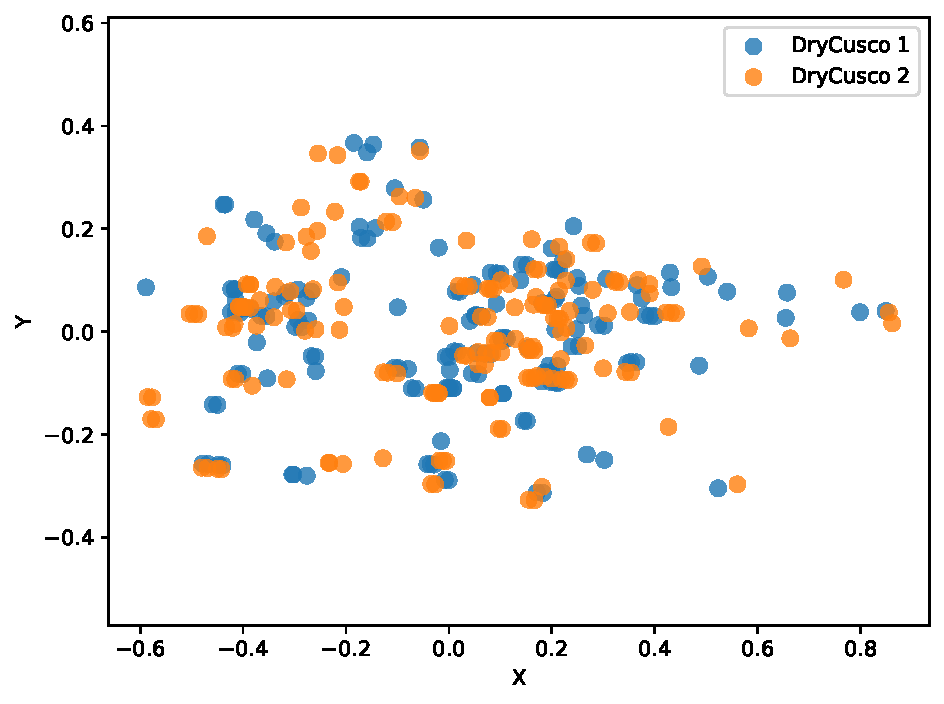
\includegraphics[
                    width=\linewidth,
                    trim=0pt 0pt 0pt 0pt, % trim: left bottom right top
                    clip
                ]{../images/node_embeddings_2d_GINE_SecoCusco.pdf}
                \caption{For Cocoa (DryCusco).}
                % \source{Author, 2024.}
            \end{subfigure}
            % \hfill
            \hspace{1cm}
            \begin{subfigure}{0.4\textwidth}
                \centering
                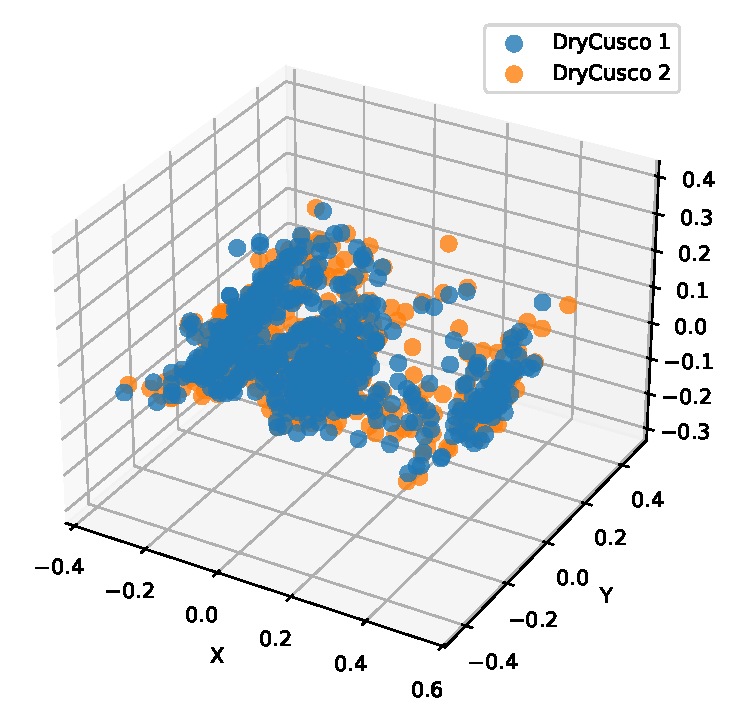
\includegraphics[
                    width=\linewidth,
                    trim=0pt 0pt 0pt 0pt, % trim: left bottom right top
                    clip
                ]{../images/node_embeddings_3d_GINE_SecoCusco.pdf}
                \caption{For Cocoa (DryCusco).}
                % \source{Author, 2024.}
            \end{subfigure}
            \caption{Node embeddings.}
            % \source{Author, 2024.}
            % \label{fig:my_image}
        \end{figure}

        \begin{note}
            {Introduce your self}
        \end{note}
    \end{frame}

    \begin{frame}{Network alignment}
        \begin{columns}[t] % Option "c" centers vertically, while "t" aligns to the top.
            \begin{column}{0.4\textwidth}
                \begin{table}[htp!]
                    \footnotesize % \scriptsize
                    \centering
                    \caption{Node alignments (DryCusco).}
                    % \label{tab:table1}
                    \begin{tabular}{rl}\toprule
                        ID 1 & ID 2 \\\midrule                        
                        0 & 93 \\
                        \rowcolor{yellow}
                        2 & 2 \\
                        4 & 57 \\
                        \rowcolor{yellow}
                        5 & 5 \\
                        7 & 93 \\
                        ... & ... \\
                        \rowcolor{yellow}
                        542 & 542 \\
                        \rowcolor{yellow}
                        551 & 551 \\
                        556 & 509 \\
                        557 & 550 \\
                        558 & 530 \\\bottomrule
                    \end{tabular}
                \end{table}
            \end{column}
            
            \begin{column}{0.6\textwidth}
                \begin{table}[htp!]
                    \footnotesize % \scriptsize
                    \centering
                    \caption{Node filtered \alert{294/559} (DryCusco).}
                    % \label{tab:table1}
                    \begin{tabular}{lrrl}\toprule
                        % ID & Rt & Mz & Metabolite name \\\midrule
                        % 2	& 0.097	& 172.95681 & Unknown \\
                        % 5	& 0.201	& 144.98254 & Unknown \\
                        % 15	& 1.871	& 118.08675 & Betaine \\
                        % 30	& 1.949	& 446.88860 & Unknown \\
                        % % 32	& 2.020	& 151.03559 & [Similar to: N-Acetyl-L-cysteine; ΔMass: -13.0... \\
                        % % 38	& 2.086	& 381.08003 & 5-({[3-chloro-5-(trifluoromethyl)-2-pyridyl]me... \\
                        % 46 &	2.110	& 118.08671	& Betaine \\
                        % 531	& 29.792	& 374.30350 & Docosahexaenoic acid ethyl ester \\
                        % 532	& 29.794	& 352.32167 & Unknown \\
                        % 537	& 29.838	& 454.42642 & N-Hexacosanoylglycine \\
                        % 538	& 29.839	& 150.12816 & 2,6-Diethylaniline \\
                        % 542	& 29.860	& 398.23344 & Drotaverine \\
                        % 551	& 29.954	& 150.12807 & 2,6-Diethylaniline \\\bottomrule
                        ID & Rt & Mz & Formula \\\midrule
                        \alert{2}	& $0.097$	& $172.95681$ & Unknown \\
                        \alert{5}	& $0.201$	& $144.98254$ & Unknown \\
                        15	& $1.871$	& $118.08675$ & $\mathrm{C_{5}H_{11}NO_2}$ \\
                        % 30	& $1.949$	& $446.88860$ & Unknown \\
                        % 32	& 2.020	& 151.03559 & [Similar to: N-Acetyl-L-cysteine; ΔMass: -13.0... \\
                        38	& $2.086$	& $381.08003$ & $\mathrm{C_{14}H_{16}ClF_{3}N_{4}OS}$ \\
                        46 & $2.110$	& $118.08671$	& $\mathrm{C_{5}H_{11}NO_{2}}$ \\
                        $\cdots$ & $\cdots$ & $\cdots$ & $\cdots$ \\
                        531	& $29.792$	& $374.30350$ & $\mathrm{C_{24}H_{36}O_{2}}$ \\
                        % 532	& 29.794	& 352.32167 & Unknown \\
                        537	& $29.838$	& $454.42642$ & $\mathrm{C_{28}H_{55}NO_{3}}$ \\
                        538	& $29.839$	& $150.12816$ & $\mathrm{C_{10}H_{15}N}$ \\
                        \alert{542}	& $29.860$	& $398.23344$ & $\mathrm{C_{24}H_{31}NO_{4}}$ \\
                        \alert{551}	& $29.954$	& $150.12807$ & $\mathrm{C_{10}H_{15}N}$ \\\bottomrule
                    \end{tabular}
                \end{table}
            \end{column}
        \end{columns}

        \begin{note}
            {Introduce your self}
        \end{note}
    \end{frame}

    % \begin{frame}{Clustering analysis}
    %     \begin{figure}[htp!]
    %         \centering
    %         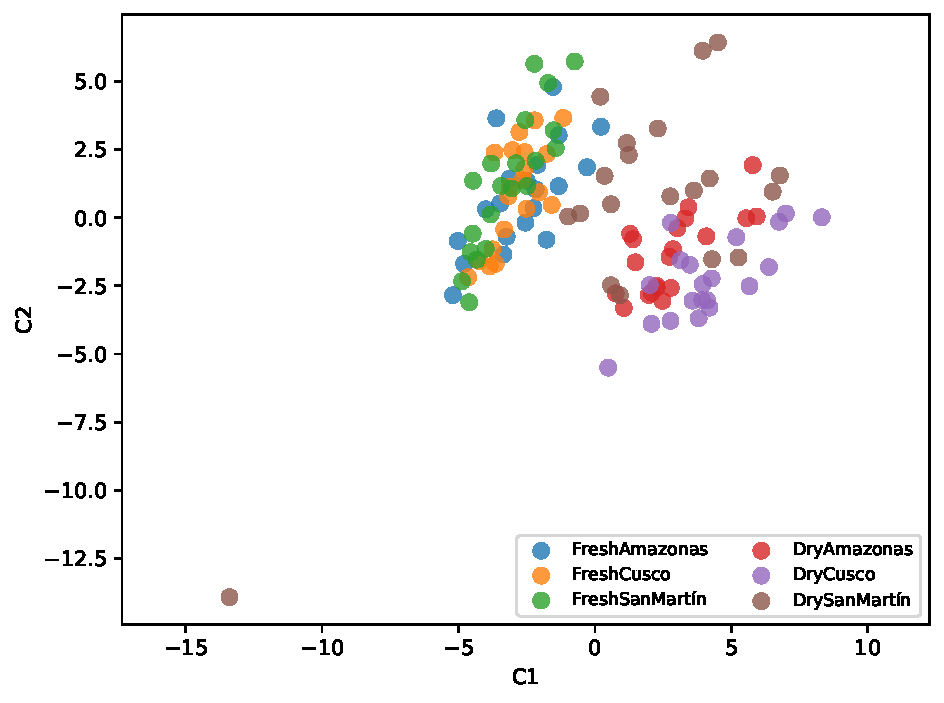
\includegraphics[
    %             width=0.6\linewidth,
    %             trim=0pt 0pt 0pt 0pt, % trim: left bottom right top
    %             clip
    %         ]{../images/clustering_GINE_SecoCusco.pdf}
    %         \caption{Clustering (DryCusco).}
    %         % \source{Author, 2024.}
    %         % \label{fig:my_image}
    %     \end{figure}

    %     \begin{note}
    %         {Introduce your self}
    %     \end{note}
    % \end{frame}

    \begin{frame}{Additional results}
        \begin{columns}[b] % Option "c" centers vertically, while "t" aligns to the top.
            \begin{column}{0.3\textwidth}
                \begin{figure}[htp!]
                    \centering
                    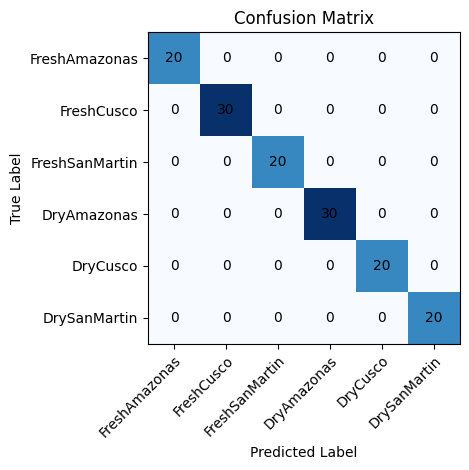
\includegraphics[
                        width=0.95\linewidth,
                        trim=0pt 0pt 0pt 0pt, % trim: left bottom right top
                        clip
                    ]{../images/cm_exp8}
                    \caption{Downstream task.}
                    % \source{Author, 2024.}
                    % \label{fig:my_image}
                \end{figure}
            \end{column}
            \begin{column}{0.7\textwidth}
                \begin{figure}[htp!]
                    \centering
                    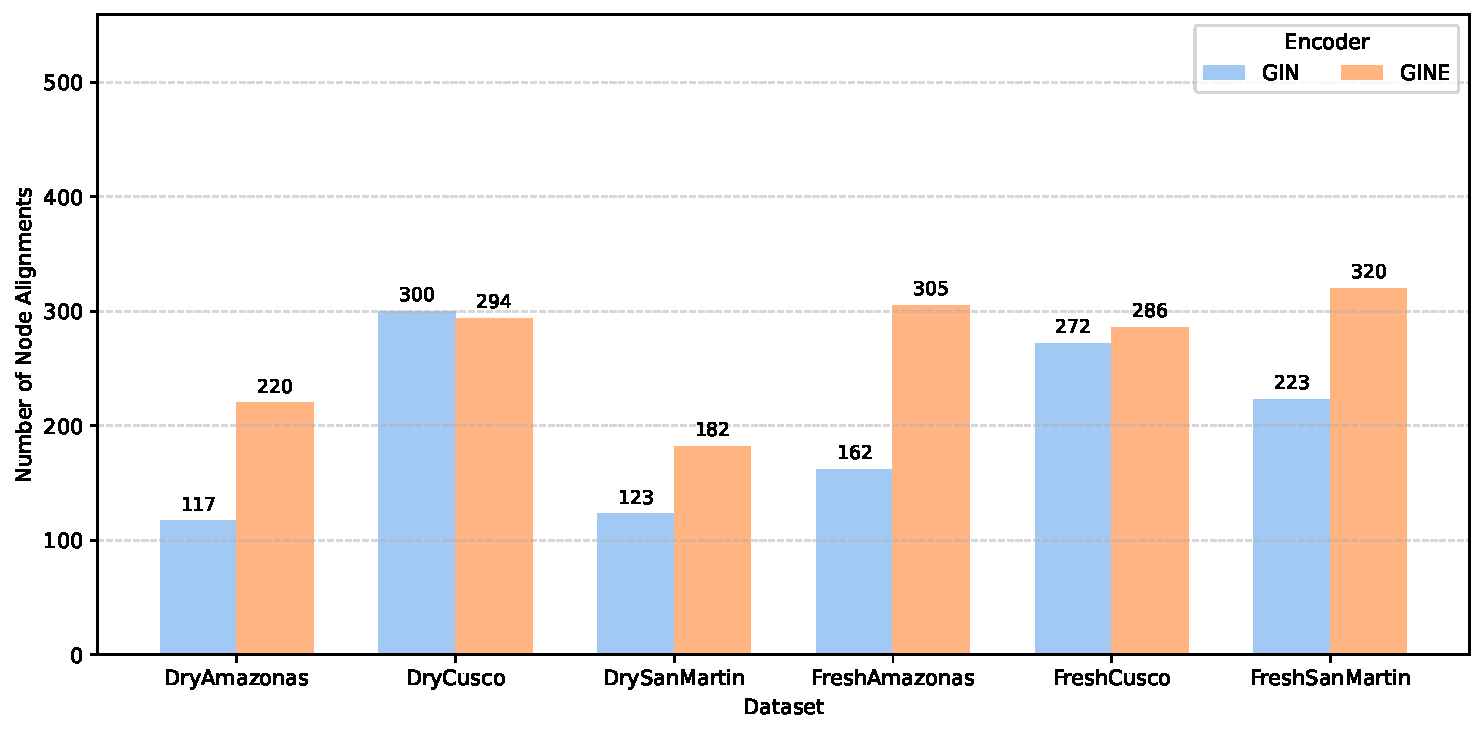
\includegraphics[
                        width=1.05\linewidth,
                        trim=0pt 0pt 0pt 0pt, % trim: left bottom right top
                        clip
                    ]{../images/number_node_alignment.pdf}
                    \caption{\texttt{GIN} vs. \texttt{GINE}.}
                    % \source{Author, 2024.}
                    % \label{fig:my_image}
                \end{figure}
            \end{column}
        \end{columns}

        

        % Include clasificación -> GIN, grano, prediction

        \begin{note}
            {Introduce your self}
        \end{note}
    \end{frame}

    % Clustering analysis
    % exp5
    % gine fresco cusco
    % gine seco cusco

% \section{Discussion}

\section{Conclusions}
    \begin{frame}{Conclusions}
        % Our proposal, is a approach to the exploratory analysis of metabolic networks.

        % Features
        \begin{itemize}
            % Significant, noise
            \item Features shared by Cocoa beans within the same group are retained, reducing the number of features before identification is attempted.
            
            % Prediction, inferencial
            \item A core graph embedding is generated for each Cocoa bean, providing a compact representation that can be used as input to a classifier for subsequent Cocoa bean identification.
            
            % Worflow, improve  (atemporal)
            \item The alignment workflow enables samples acquired on different days to be integrated into a single dataset. This approach mitigates known batch effects, such as retention-time shifts, while the graph embedding favors correlations among signals rather than depending on their absolute intensity values.
            
            % \item We designed a pipeline for a metabolomic study. \texttt{GEMNA} consists of three steps: \textit{network generation}, \textit{network filtering}, and \textit{similarity analysis}.

            % \item We evaluated the execution time for generating node embeddings and edge embeddings. The experiments demonstrate that \texttt{DGI} model is faster than \texttt{VGAE}, \texttt{LVGAE}, \texttt{ARGVA}, to generate node embeddings. % using node embeddings (based on GNN), edge embeddings, and anomaly detection algorithm.

            % \item Experiments show that our \texttt{GEMNA} is an improvement over traditional statistical-based techniques. The evaluation by silhouette score reported that \texttt{GEMNA} obtained $0.41$, meanwhile, the statistical method obtained $-0.004$. % For example, for the Mentos candy dataset, the data clusters produced by \texttt{GEMNA} were better than the ones used in traditional techniques based on statistics. \texttt{GEMNA} has $silhouette\:score = 0.409$, \textit{vs} the traditional approach has $silhouette\:score = -0.004$.

            % \item We developed a web application for metabolomic network analysis and the source code is available on GitHub.
        \end{itemize}

        \begin{note}
            {Write your notes here}
        \end{note}
    \end{frame}

% \begin{frame}{Future works}
%     Based on these results, I recommend analyzing metabolomic networks using \textit{Geometric Graph Neural Networks} (GGNN) models.

%     These models create node embeddings using the graph structure, node and edge features, and a feature tensor that helps infer the position of each metabolite within the network.
    
%     \begin{note}
%         {Write your notes here}
%     \end{note}
% \end{frame}

\section*{References}
    \begin{frame}
        \begin{center}
            {\LARGE\calligra Thanks!} \\
            % {\Huge\textit{Thank you for your attention!}}\\
            {\Huge $\infty$} \\
            % edwin.alvarez@pucp.edu.pe \\
            % \url{https://github.com/win7}
            \begin{figure}[htp!]
                \centering
                
\includegraphics[
                    width=0.07\linewidth,
                    trim=0pt 0pt 0pt 0pt, % trim: left bottom right top
                    clip
                ]{../images/qr_link.png}
                % \caption{Metabolomics workflow.}
                % \source{\cite{putri2014mass}} 
                % \label{fig:my_image}
            \end{figure}

        \end{center}

        \begin{center}
            {\LARGE Acknowledgments} \\
            \footnotesize Financial support was provided by \texttt{CONCYTEC-Prociencia} through project PE501086715-2024-PROCIENCIA. Also, I gratefully acknowledge the Pontificia Universidad Católica del Perú (\texttt{PUCP}) for the financial support provided for conference registration.
        \end{center}

        \begin{figure}
            \centering
            \begin{subfigure}{0.18\textwidth}
                \centering
                
\includegraphics[
                    width=\linewidth,
                    trim=0pt 50pt 0pt 50pt, % trim: left bottom right top
                    clip
                ]{../images/PUCP_logo.png}
                % \caption{My image.}
                % \source{Author, 2024.}
            \end{subfigure}
            % \hfill
            \hspace{1cm}
            \begin{subfigure}{0.18\textwidth}
                \centering
                
\includegraphics[
                    width=\linewidth,
                    trim=0pt 130pt 0pt 150pt, % trim: left bottom right top
                    clip
                ]{../images/PROCIENCIA-LOGO.png}
                % \caption{My image.}
                % \source{Author, 2024.}
            \end{subfigure}
            % \caption{My image.}
            % \source{Author, 2024.}
            % \label{fig:my_image}
        \end{figure}

        \begin{figure}[htp!]
                \centering
                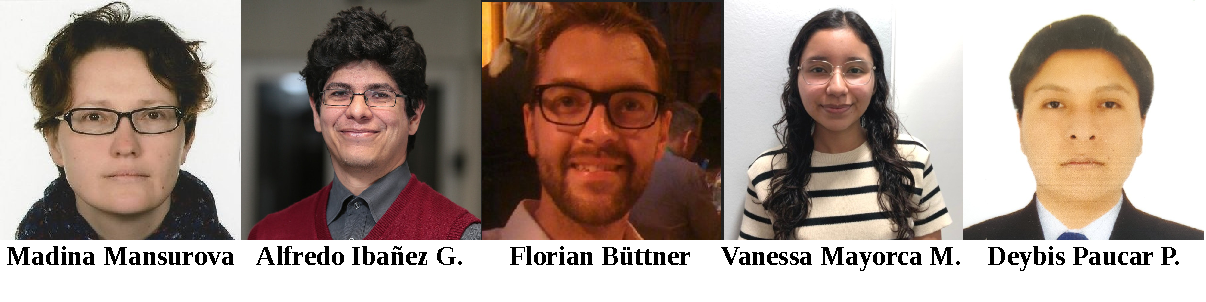
\includegraphics[
                    width=0.65\linewidth,
                    trim=0pt 0pt 0pt 0pt, % trim: left bottom right top
                    clip
                ]{../images/teams.pdf}
                % \caption{Metabolomics workflow.}
                % \source{\cite{putri2014mass}} 
                % \label{fig:my_image}
            \end{figure}

    \end{frame}
    
    % Bibliography
    % \input{ref.bib}
    % \begin{frame}[allowframebreaks]
    %     \footnotesize % use this command to resize
    %     \bibliography{ref}
    %     \bibliographystyle{unsrt}
    %     % \bibliographystyle{alpha}
        
    %     % \begin{itemize}
    %     %     \item Erciyes, K. (2018). \textit{Guide to graph algorithms} % (pp. 15-35). Springer International Publishing.
    %     %     \item Yao Ma, Jiliang Tang. (2021). \textit{Deep Learning on Graphs}.
    %     %     \item Stamile C., Marzullo A., Deusebio E. (2021). \textit{Graph Machine Learning}.
    %     %     \item Wu, L., Cui, P., Pei, J., Zhao, L., \& Guo, X. (2022). \textit{Graph neural networks: foundation, frontiers and applications}. % In Proceedings of the 28th ACM SIGKDD conference on knowledge discovery and data mining (pp. 4840-4841).            
    %     %     % \item Knickerbocker D. (2023). \textit{Graph Network Science with Python}.
    %     %     \item Knickerbocker, D. (2023). \textit{Network Science with Python}. % Packt Publishing Ltd.
    %     %     \item Labonne, M. (2023). \textit{Hands-On Graph Neural Networks Using Python}.
    %     %     \item Broadwater, K., \& Stillman, N. (2025). \textit{Graph neural networks in action}. % Simon and Schuster.
    %     % \end{itemize}
    % \end{frame}
\end{document}